\documentclass[11pt, a4paper, oneside]{article}

\usepackage[francais]{babel}
\usepackage[T1]{fontenc}
\usepackage[utf8]{inputenc}

\usepackage[left=2cm, right=2cm, top=2cm, bottom=2cm]{geometry}
\usepackage{fancyhdr}
\usepackage{lastpage}
\usepackage{hyperref}

\usepackage{graphicx}
\usepackage{tikz}
\usepackage{pgfgantt}

\usepackage{perpage} %the perpage package
\MakePerPage{footnote} %the perpage package command

\usepackage{color}
\usepackage{colortbl}

\usepackage{makeidx}

\usepackage{listings}
\usepackage{CJKutf8}

\makeindex
\makeatletter
\renewenvironment{theindex}
{
    \thispagestyle{fancy}
    \setlength{\parindent}{0pt}
    \let
    \item
    \@idxitem
}{\onecolumn}
\makeatother

\setlength{\parindent}{0cm}

\lstset{
    basicstyle=\ttfamily,
    stringstyle=\ttfamily\color{green!50!black},
    keywordstyle=\bfseries\color{blue},
    commentstyle=\itshape\color{red!50!black},
    showstringspaces=true,
    tabsize=4,
    frame=single,
    numbers=left,
    numberstyle=\tiny,
    firstnumber=1,
    stepnumber=1,
    numbersep=5pt,
    breaklines=true
}

\graphicspath{{img/}}

\pagestyle{fancy}
\setlength{\headheight}{14pt}
\renewcommand{\headrulewidth}{0.5pt}
\lhead{Yannick Brodard}
\chead{}
\rhead{\today}
\renewcommand{\footrulewidth}{0.5pt}
\lfoot{CFPT - École d'informatique}
\cfoot{Étude de Unreal Engine 4}
\rfoot{Page \thepage ~sur \pageref{LastPage}}

% Niveau table des matières
\setcounter{tocdepth}{3}

% ---------------------------------------------------------------------
\begin{document}
\begin{center}
{\Huge{Étude de Unreal Engine 4}} \\[0.5cm]
{\LARGE{Travail de semestre}}\\[0.5cm]
{\Large{Yannick Brodard}}\\[0.3cm]
\today\\

\includegraphics[scale=0.4]{UE4_logo}
\end{center}
Enseignants :
\begin{itemize}
\item Christophe Maréchal
\item Stéphane Garchery\\[3cm]
\end{itemize}
\textbf{CFPT - École d'informatique}\\
Technicien ES 2\textsuperscript{ème} année
\thispagestyle{empty}
\newpage
\vspace*{\fill}
\textit{Most good programmers do programmingnot because they expect to get paid or get adulation by the public, but because it is fun to program.}

- Linus Torvalds
\vspace*{\fill}
\thispagestyle{empty}
\newpage
\part{Avant-propos}
\section{Résumé}
% A COMPLETER A LA FIN
\section{Remerciements}
% A COMPLETER A LA FIN
\newpage
\tableofcontents
\newpage
\part{Introduction}
\section{Définition du projet}
Ce projet a été mis en place pour s'initier au développement de jeux-vidéos avec un moteur de jeu, étant donné que mon travail de diplôme sera de développer un jeu complet.

Pour se faire, une étude et un travail pratique avec l'environnement Unreal Engine 4 a été proposée.

Dans cette étude, plusieurs aspects de ce moteur seront analysés et documentés, notamment :
\begin{itemize}
\item La gestion des modèles 3D
\item La création de jeu
\item L'interaction utilisateur-machine\\
\end{itemize}
Proposé par Monsieur Maréchal, l'intégration d'un périphérique 3D (le \textit{Novint Falcon 3D Touch Controller}) a été prévu pour étudier son fonctionnement et son implémentation sur ce genre d'environnement.
\subsection{Unreal Engine 4}
\label{sec:ue4definition}
Unreal Engine est un moteur de jeu développé par Epic Games\footnote{\url{http://epicgames.com/}} qui a été présenté pour la première fois en 1998 avec un jeu FPS\footnote{First Person Shooter : Jeu de tir à la première personne} nommé \textit{Unreal}. Bien que le moteur était développé principalement pour des jeux FPS, il est aujourd'hui utilisé pour beaucoup d'autres genres de jeux comme :
\begin{itemize}
\item Infiltration
\item Action
\item MMO (Jeux massivement multijoueurs en-ligne)
\item Jeux à la troisième personne
\item Et bien d'autres...
\end{itemize}
La version actuelle de UE4\footnote{Unreal Engine 4} est conçu pour Microsoft DirectX 10 à 12, OpenGL et JavaScript/WebGL.
\newpage
\section{Définition des objectifs}
Le but est d'étudier l'environnement de Unreal Engine 4 dans ses détails, c'est-à-dire la programmation avec UE4, la modélisation, l'édition de différents scénarios et prise en main de la physique du moteur. Un travail avec la souris \textit{Novint Falcon 3D Touch Controller} est aussi demandé, cette souris 3D permet à l'utilisateur de reproduire des mouvement sur 3 axes qui peuvent être interprétées par l'ordinateur.

\begin{figure}[h]
	\begin{center}
	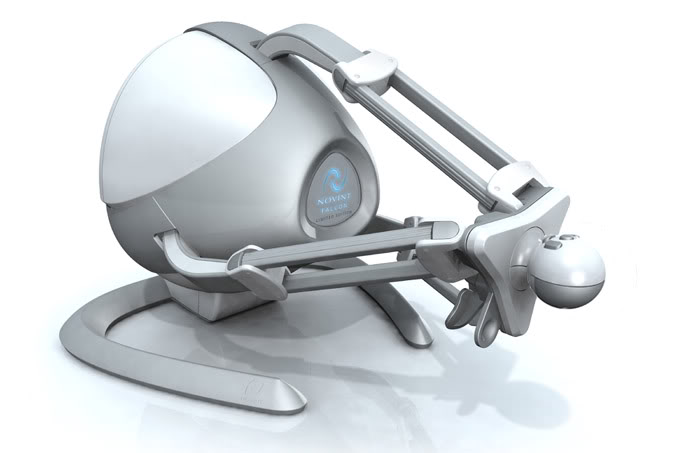
\includegraphics[scale=.4]{falcon}
	\caption{Souris Novint Falcon 3D Touch Controller}
	\end{center}
\end{figure}

Une étude comparative du moteur de jeu sera faite avec le moteur Unity 3D, cette étude est confiée à Monsieur Daniel Lopes.\\[0.3cm]
Le mini-jeu est basé sur le jeu \textit{Galaga}. Dans ce jeu 2D, l'utilisateur contrôle un vaisseau qui peut se déplacer sur les axes x et y. Des vagues de vaisseaux ennemis se positionnent devant le joueur pour tenter de l'éliminer. Ils se positionnent en groupe et tir sur le joueur. Le joueur doit faire de son mieux pour esquiver les tirs et doit détruire tous ses ennemis.

\begin{figure}[h]
	\begin{center}
	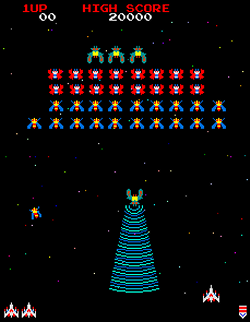
\includegraphics[scale=0.8, angle=90]{Galaga}
	\caption{Un capture d'écran du jeu Galaga (Orienter à 90\degre)}
	\end{center}
\end{figure}

\newpage
\part{Analyse préliminaire}
\section{Analyse de l'existant}
Concernant le mini-jeu, il y a la plateforme et le moteur sur le quel celui-ci se repose. Unreal Engine 4 permet de développer des jeux de manière beaucoup plus rapide et efficace sans ré-inventer la roue. Ceci permet d'éviter d'écrire des librairie pour, par exemple, gérer l'affichage du jeu.

À propos du jeu en lui-même, il n'y a rien de codé ni préparé. Il y a la conception totale à faire.
\section{Environnement de travail}
\subsection{Logiciel}
\begin{itemize}
\item Unreal Engine 4\footnote{Pour en savoir plus sur Unreal Engine 4 voir la section \ref{sec:ue4definition} sur la page \pageref{sec:ue4definition}.}
\item Outils de Unreal Engine 4\\
\end{itemize}
\subsection{Matériel}
\begin{itemize}
\item PC 1x
	\begin{itemize}
	\item 1024MB NVIDIA GeForce GTX 550 Ti
	\item Intel Core i7 2600K @ 3.40GHz
	\item ASUSTeK Computer INC. P8Z68-V LE
	\item 8.00 Go Dual-Channel DDR3 @ 824MHz
	\end{itemize}
\item Écran 2x
\item Clavier 1x
\item Souris 1x
\end{itemize}
\subsection{Conditions de travail}
\subsubsection{Durée}
Le projet se déroulera sur 48 heures de cours, séparée sur 12 jours et 4 périodes par jour. C'est-à-dire, une fois par semaine, le mercredi matin, 4 périodes seront dédiées à ce projet. Il est aussi possible de travailler sur le projet en dehors des ces tranches horaires.
\subsubsection{Délivrables}
\begin{itemize}
\item Un journal de bord
\item Une copie de la documentation
\item Un poster qui présente le projet
\item La documentation et la source du projet seront déposées sur la plateforme Moodle du CFPT-EI.
\end{itemize}
\subsubsection{Suivi}
Ce projet sera évalué et suivi par Monsieur Christophe Maréchal et Monsieur Stéphane Garchery.
\newpage
\part{Étude}
\newpage
\part{Analyse fonctionnelle - Jeu}
\newpage
\part{Analyse Organique - Jeu}
\newpage
\part{Résultats}
\section{Tests}
\section{Conclusion}
\newpage
\part{Annexes}
\section{Planning}
\subsection{Initial}
\begin{figure}[h]
	\begin{center}
	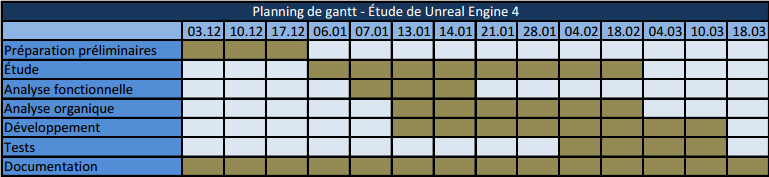
\includegraphics[scale=.924, angle=90]{planninggantt}
	\caption{Planning initial du projet}
	\label{planningintial}
	\end{center}
\end{figure}
\newpage
\subsection{Réel}
\end{document}